\documentclass[12pt,a4paper]{report}
\usepackage[utf8]{inputenc}
\usepackage[T1]{fontenc}
\usepackage{lmodern}
\usepackage{geometry}
\geometry{margin=1in}
\usepackage{setspace}
\onehalfspacing
\usepackage{amsmath, amssymb}
\usepackage{graphicx}
\usepackage{booktabs}
\usepackage[hidelinks]{hyperref}
\usepackage{natbib}
\usepackage{float}
\usepackage{tabularx}
\bibliographystyle{chicago}

\begin{document}

\begin{titlepage}
\centering
{\Large CHARLES UNIVERSITY}\\
\vspace{1em}
{\large Faculty of Social Sciences}\\
\vspace{2em}
{\LARGE \textbf{Risk Channels in Monetary Policy}}\\
\vspace{1em}
{\large A Quantitative Economics Approach}\\
\vfill
Master's Thesis
\vspace{2em}

Author: Boris Gerát\\
Supervisor: [Your Supervisor]\\
Year of Defence: 2026
\end{titlepage}

\chapter*{Declaration}
I hereby declare that I have completed this thesis independently using only the listed sources.

\vspace{2em}
In Prague, [date]\\
Boris Gerát

\chapter*{Abstract}
[Write abstract here]

\chapter*{Keywords}
Risk, Monetary policy, BVAR, Financial sector

\tableofcontents
\newpage

\chapter*{Introduction}
\addcontentsline{toc}{chapter}{Introduction}
[Write introduction here]

\chapter{Data and Methodology}
This chapter presents the data sources and empirical methodology used in the analysis. 
\section{Data}

Data is an essential part of this empirically based thesis. The work leverages time series from multiple
sources, and because of this, I divide this section into multiple parts. Each subsection addresses a
specific component of the dataset in relation to the corresponding data source used in that part of
the analysis. I begin with sectoral-level variables, then proceed to off-the-shelf risk indices, and
finally to self-collected data used for constructing custom risk indices.

\subsection{Financial Sector Variables}

The main objective when selecting sectoral-level variables was to identify a set of variables that
would be comparable across all sectors. This initially proved difficult due to fragmented data
sources, mismatched time windows, and differences in reporting frequencies across the three
subsectors.

The banking sector did not pose a significant issue in this regard, as it is one of the most
regulated and well-documented sectors. As the primary data source for the banking sector, I use data
from the Federal Deposit Insurance Corporation (FDIC), which provides a rich and easily accessible
database of balance sheet information for the banking system. Data for this sector was collected
first, and the broader availability of variables guided the design and selection of variables for
the remaining sectors. While this subsector imposed the fewest constraints on the scope of the
research, the final variable set still had to be reduced to ensure comparability with the other two
sectors.

For the shadow banking subsector, I use the Z.1 Financial Accounts of the United States, which, to
my knowledge, represent one of the most comprehensive sources for this segment of the financial
system. Specifically, I use the component labeled ``Other financial busenises,'' denoted in L.132 which is constructed by subtracting the
banking and hedge fund subsectors (reported separately) from the broader financial accounts. This
aggregate captures the activity and balance sheet conditions of entities such as money market
funds, mutual funds, holding companies, and issuers of asset-backed securities. Initially, I
intended to provide two perspectives on the shadow banking sector: one based on the aggregate
``Other'' category and another focusing on its largest component, money market funds. However,
disaggregated data for specific entities were not sufficiently aligned with the structure of the
banking sector data. As a result, I focus exclusively on the aggregate representation. An important
implication of using this source is that the analysis is restricted to quarterly frequency, as the
Z.1 Financial Accounts are published only on a quarterly basis.

The final subsector considered is the hedge fund sector. The regulatory framework governing the
reporting of this subsector is relatively recent, and the data can be found in releases associated
with the H.8 financial accounts. The structure of reporting and the available variables are similar
to those in the Z.1 accounts. However, due to the recent introduction of these reporting standards,
data for hedge funds begin only in 2012 Q4. This represents a substantial limitation compared to the
banking and shadow banking sectors, which are available from 1997 Q1. Restricting all sectors to the
shorter hedge fund sample would significantly reduce the scope of the analysis. Therefore, I retain
the 1997 Q1 -- 2024 Q4 window for the banking and shadow banking sectors, while reporting hedge fund
results starting from 2012 Q4. Comparisons involving the hedge fund sector must therefore be
interpreted with caution, as earlier episodes such as the dot-com bubble or the global financial
crisis are not captured in its sample.
\begin{table}[H]  % forces placement HERE
\centering
\renewcommand{\arraystretch}{2.8} % vertical spacing
\begin{tabular}{l|c} % second column centered
\hline
\textbf{Variable} & \textbf{Fraction} \\
\hline
Wholesale Funding & $\dfrac{\text{Brokered Deposits + Other Borrowed Money}}{\text{Total Assets}}$ \\
\hline
Liquidity Buffer  & $\dfrac{\text{Cash + Treasuries}}{\text{Total Assets}}$ \\
\hline
Capital Cushion   & $\dfrac{\text{Total Equity}}{\text{Total Assets}}$ \\
\hline
Number of Loans  & -- \\
\hline
\end{tabular}
\caption{This constructed balance sheet ratios are used in the main BVAR analysis and serve as the basis for observing impulse response function reactions to increases in risk, which are discussed later in the study.}
\end{table}

In Table~1.1, the variables that were consistently collected across all subsectors are presented.
The number and variety of these variables allow me to construct ratio-based measures that combine
multiple balance sheet components through their interactions. This transformation reduces the
dimensionality of the system, which is particularly important given the relatively short time
dimension of the dataset used in the BVAR model.

Wholesale funding captures the extent to which a given subsector relies on market-based financing
and access to capital markets. The liquidity buffer reflects the share of balance sheet resources
allocated to highly liquid assets, providing a measure of short-term resilience to funding shocks.
The capital cushion serves as a proxy for leverage, indicating the degree of risk-taking behavior
within the subsector. The number of loans as they are as it carries
substantial informational content on its own and directly captures credit provision dynamics.

This broader set of variables is designed to capture the overall behavior of each subsector when
subject to monetary policy and risk shocks. At the same time, the selection enables internal
consistency checks and robustness in the analysis of impulse response functions. For instance,
changes in leverage should be accompanied by corresponding movements in wholesale funding, which
provides an additional layer of validation for the identified transmission mechanisms.

\subsection{Monetary Policy Variable}
For the role of the main monetary policy variable, I considered multiple candidates and approaches.
However, for the final analysis, I choose to use the shadow rate proposed by Wu and Xia (2016).
This measure provides a more accurate representation of the stance of monetary policy when the
effective federal funds rate is constrained by the zero lower bound.

During the Global Financial Crisis, monetary policy became highly accommodative and relied on
non-standard tools such as quantitative easing alongside conventional rate setting. These measures
are not fully captured by the standard effective federal funds rate, as nominal interest rates are
bounded at zero and cannot reflect additional monetary accommodation. The Wu and Xia shadow rate
addresses this limitation by allowing for negative values, thereby capturing the implicit policy
stance under unconventional monetary policy. At the same time, it closely tracks the effective
federal funds rate during periods away from the lower bound, ensuring consistency across regimes.

This methodology is particularly useful during and immediately after the 2008 financial crisis.
However, once the shadow rate converges back to the official effective federal funds rate in more
stable periods, the difference between the two becomes negligible. As the shadow rate series is not
available after 2023, and re-estimating the model for a relatively short extension of the sample is
not essential for the purposes of this analysis, I replace the missing observations with the
effective federal funds rate. Given the close co-movement of the two series outside of the
zero-lower-bound period, this substitution does not materially affect the results.

Initially, I also considered the methodology of Romer and Romer (2004), which isolates unexpected
monetary policy shocks by removing the anticipated component of policy changes. This approach is
useful in settings where expectations may bias the estimated effects of monetary policy, for
example through the so-called price puzzle. However, given the lower frequency of the data used in
this analysis, such issues are less pronounced. In this context, the shadow rate approach provides a
more suitable measure of the overall stance of monetary policy and is therefore preferred.

\subsection{Benchmark Risk Indicies}

To measure effcts of my custom risk indcies I am intorudicng large quantiiyfo bencahmrk risk idncie
both from tradioanl time series based kinds and from sentiemnt ones too. In this way even if the
custom risk idncies will fail to deliver effect the BVAR analysis that rleis on them will still be
valubale. The sued risk idncies can see be listed in the table bellow with their shortcus used in
analysiis and resutls and short explanation. 

\begin{table}[H]
\centering
\caption{Financial Risk and Uncertainty Indices}
\label{tab:risk_indices}

\vspace{0.3cm}
\renewcommand{\arraystretch}{1.4}

\begin{tabularx}{\textwidth}{p{2.5cm} p{6.5cm} X}
\hline
\textbf{Abbreviation} & \textbf{Full Name} & \textbf{Description} \\
\hline

STLFSI & St. Louis Fed Financial Stress Index 
& Composite index constructed from 18 financial market variables, including interest rate spreads, volatility measures, and yield curve indicators. \\
\cline{1-3}

NFCI & Chicago Fed National Financial Conditions Index 
& Broad index based on over 100 financial indicators capturing risk, credit, and leverage conditions in the U.S. financial system. \\
\cline{1-3}

KCFSI & Kansas City Financial Stress Index 
& Stress index constructed from 11 financial variables, focusing on yield spreads and market volatility across financial sectors. \\
\cline{1-3}

VIX & CBOE Volatility Index 
& Market-based measure of expected volatility derived from S\&P 500 option prices; commonly interpreted as a forward-looking risk indicator. \\
\cline{1-3}

EPUI & Economic Policy Uncertainty Index 
& News-based index measuring policy-related economic uncertainty using frequency of newspaper articles combined with policy indicators. \\
\cline{1-3}

NSI & News Sentiment Index (Shapiro et al.) 
& Text-based sentiment index constructed from news articles, capturing positive and negative economic tone across a large corpus of media sources. \\

\hline
\end{tabularx}

\vspace{0.2cm}
\begin{flushleft}
\footnotesize
\textit{Note:} The indices combine financial market data and textual information to capture different dimensions of risk and uncertainty relevant for macro-financial analysis.
\end{flushleft}

\end{table} 

In the majority of related studies, the STLFSI (often referred to simply as the Financial Stress Index, FSI) serves as a primary proxy for financial risk, typically alongside the VIX index. Together, these two measures provide a robust framework for analyzing risk responses. The STLFSI captures broad financial stress conditions, while the VIX represents a purely market-based measure derived from S\&P 500 option prices, reflecting forward-looking expectations of volatility.

However, in this analysis, I extend the set of risk indicators by incorporating additional indices constructed by Federal Reserve Banks beyond the St. Louis Fed. In particular, I include the NFCI and KCFSI, which differ in their construction methodologies relative to the STLFSI. The NFCI can be viewed as a higher-dimensional measure, incorporating a large number of financial variables to capture a broader range of risk, credit, and leverage conditions. In contrast, the KCFSI adopts a more parsimonious approach, focusing on a smaller set of variables closely linked to financial market volatility and stress dynamics.

In addition to financial stress indices, I incorporate sentiment-based measures of risk. The Economic Policy Uncertainty Index (EPUI) is included as it is explicitly designed to capture uncertainty in the economic and policy environment through a structured, news-based methodology. In contrast, the Shapiro News Sentiment Index serves a more general purpose, capturing overall economic tone in news coverage. As such, while it provides valuable information, it does not exclusively target risk or uncertainty in the same way as EPUI.

Overall, this set of risk indices provides a broad and complementary representation of financial risk and uncertainty. It enables a more comprehensive assessment of the risk channel and facilitates robustness checks within the BVAR framework, particularly when compared to the custom risk indices constructed in this study.

\subsection{Custom Risk Indicies}
In this thesisi I am intorudicng three types of risk indcies. First type is time sries absed simail
to the risk icnies created by federal reserve banks. Second type are risk idncies are absed on
textual data which si then trnformed into sentiment simailry as Shapiro news index and EPU index.
The last type is the combination of them, to try leverage signals from both. 

\subsubsection{Time Series Based Indecies}

To construct the custom risk index, I follow the general methodology employed by the Federal Reserve Bank of St. Louis in the development of financial stress indices. This approach is based on selecting variables that exhibit a strong signal with respect to financial risk and extracting their common component through principal component analysis.

In this thesis, I extend this methodology by introducing a hierarchical factor structure. Specifically, I first group variables according to the type of signal they capture, ranging from policy-related indicators to market-based measures. Within each group, I extract the first principal component, which represents the dominant common movement specific to that category of variables.

In the second stage, I take the first principal component of these group-level factors. This results in a final aggregate factor that captures the common variation across all signal types. In this way, the constructed risk index reflects a broad and integrated measure of financial risk, incorporating information from multiple dimensions of the financial system.

All variables included in the construction of the index are listed below. 

\begin{table}[H]
\centering
\caption{Variables Used in Hierarchical Risk Factor Construction}
\label{tab:hierarchical_risk_variables}

\vspace{0.3cm}
\renewcommand{\arraystretch}{1.4}

\begin{tabular}{p{3cm} p{10cm}}
\hline
\textbf{Category} & \textbf{Variables} \\
\hline

Credit 
& Moody’s Baa Corporate Bond Spread, \\
& ICE BofA US High Yield Spread, \\
& ICE BofA US Corporate Bond Spread \\
\cline{1-2}

Funding 
& Commercial Paper Spread, \\
& Prime Rate Minus Federal Funds Rate, \\
& Commercial Paper Minus 3-Month Treasury Spread \\
\cline{1-2}

Policy 
& 10Y--2Y Treasury Spread, \\
& 10Y--3M Treasury Spread, \\
& 10Y Treasury Minus Federal Funds Rate \\
\cline{1-2}

Market 
& NASDAQ Composite Index (log returns), \\
& S\&P 500 Index (log returns), \\
& Russell Index (log returns) \\
\hline

\end{tabular}

\vspace{0.2cm}
\begin{flushleft}
\footnotesize
\textit{Note:} Variables are grouped according to their economic interpretation into credit risk, funding conditions, monetary policy stance, and market-based indicators. Within each group, the first principal component is extracted and subsequently aggregated into a final risk factor.
\end{flushleft}

\end{table}

The choice of variables was straightforward, as the objective was to achieve results comparable to existing Federal Reserve risk indices. This ensures that the constructed index remains methodologically comparable to established benchmarks, while still distinguishing itself through its specific variable selection and the use of hierarchical factor extraction.

\subsubsection{Sentiment Based Indecies}

In this section I want ot intorduce textal based data taht were collected from relevant soruces that
sohuld carry information about risk and confidence of the US economy. All coleaction was done by me
using legal webscraping methods. The selection of texutal sentiemnt soruces can be seen in figure 
bellow. 

\begin{figure}[H]
\centering
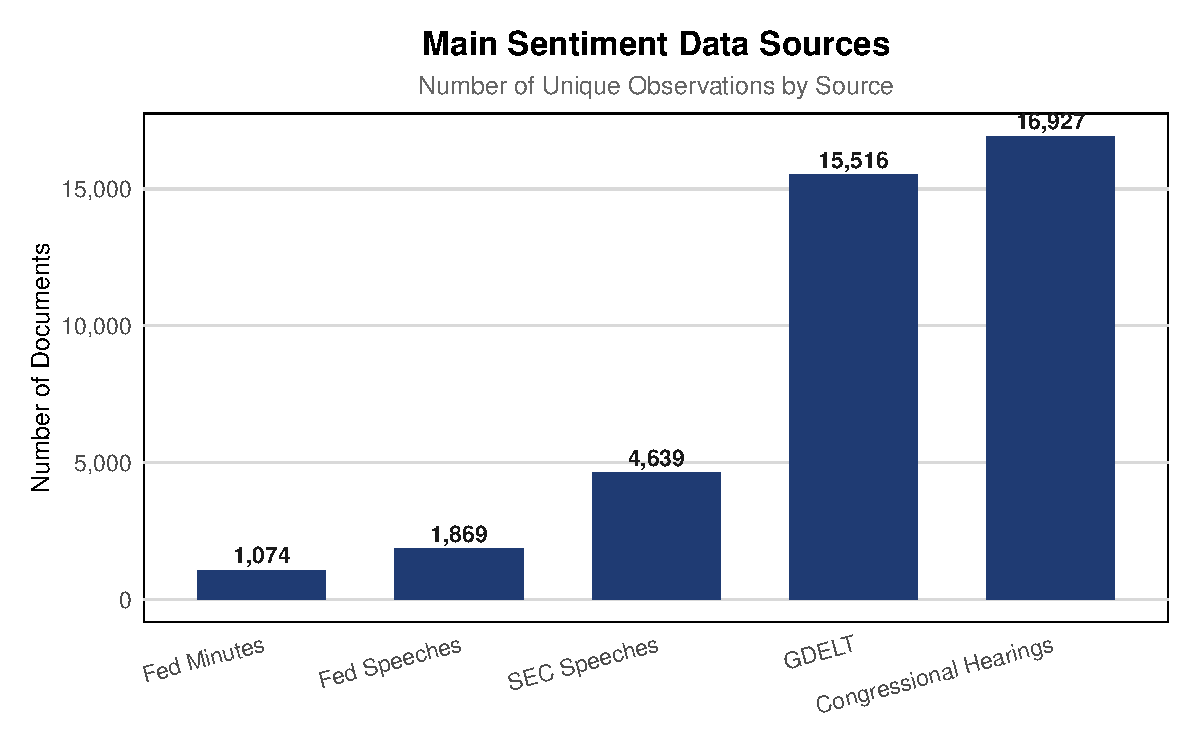
\includegraphics[width=1\textwidth]{pics/plot.pdf}
\caption{Main Sentiment Data Sources}
\label{fig:sentiment_sources}
\end{figure}

As can be seen, the sentiment index is constructed from a diverse set of textual data sources. 
The largest contribution comes from congressional hearings, filtered to include only economically 
relevant committees. The second-largest source is the GDELT project, which represents one of the 
most extensive collections of global news events. While GDELT does not provide direct access to the 
full textual content, it offers pre-constructed indices derived from news coverage. In this analysis, 
only economically relevant entries are selected.

The remaining sources are smaller in volume but provide highly relevant economic information. These 
include Securities and Exchange Commission (SEC) speeches, Federal Reserve minutes, and Federal 
Reserve speeches. Although these datasets are more limited in size, they are closely aligned with 
economic policy and institutional communication, and therefore contain strong informational content 
for sentiment extraction.

Overall, the dataset is more heavily weighted toward policy-based sources of sentiment. However, the 
inclusion of GDELT news data helps balance this by incorporating broader media-based information. 
Initially, I intended to further expand the dataset by including textual data from platforms such as 
Reddit and X (formerly Twitter). However, access to X data requires paid subscriptions, which are 
beyond the scope of a master’s research budget. In the case of Reddit, although large historical 
datasets are available through archived sources, the data collection process proved to be 
computationally intensive given the available hardware constraints. Despite these limitations, such 
data sources represent a promising extension and could further enhance the sentiment analysis.

The final sentiment measure combines this text-based index with the time-series-based risk indices. 
This is achieved through the extraction of their first principal component, consistent with the 
methodology applied throughout this thesis. In this way, the resulting index captures both 
high-frequency textual sentiment and broader macro-financial dynamics.

\section{Methodology}
In this section, I present the methodological framework and identification strategies used in this thesis. I begin with factor models for dimensionality reduction, then proceed to sentiment extraction methods, and conclude with the specification of the Bayesian VAR (BVAR) model.

\subsection{Expectation Maximization Principal Component Analysis (EMPCA)}

Based on prior experience with similar research problems, I choose to use the EMPCA model. 
This approach is both simple and powerful. Its main advantage lies in its ability to handle missing 
data through the expectation–maximization procedure, while maintaining a linear and fully 
interpretable structure. Unlike more complex nonlinear methods, EMPCA preserves transparency in the 
estimation process, which is desirable in an empirical setting.

In this thesis, EMPCA is used whenever extraction of the first principal component is required, 
forming a core building block of the hierarchical factor construction. The EMPCA follows original
methodology proposed by S. Roweis (1998).

Alternative approaches were also considered. In particular, the NIPALS algorithm and Dynamic Factor 
Models (DFM) were evaluated. However, NIPALS either underperformed relative to EMPCA or produced 
very similar results without additional benefits. Dynamic Factor Models, on the other hand, 
encountered convergence issues when applied to datasets with low dimensionality and relatively 
short time series. For these reasons, EMPCA is selected as the primary method throughout the thesis.

\subsubsection*{EMPCA Model Specification}

The EMPCA framework assumes that the observed data matrix \( X \in \mathbb{R}^{T \times N} \) can be represented by a low-dimensional factor structure:

\begin{equation}
X = W Z + \varepsilon
\end{equation}

where \( W \in \mathbb{R}^{T \times k} \) contains the latent factors, \( Z \in \mathbb{R}^{k \times N} \) are the factor loadings, and \( \varepsilon \) is an idiosyncratic error term.

\vspace{0.3cm}

The estimation proceeds via the Expectation–Maximization algorithm.

\paragraph{E-step (Expectation)}

Given current estimates of loadings \( Z^{(t)} \), the latent factors are updated as:

\begin{equation}
W^{(t+1)} = X Z^{(t)\top} \left( Z^{(t)} Z^{(t)\top} \right)^{-1}
\end{equation}

\textit{Step interpretation:}  
This step estimates the latent factors \( W \) by projecting the observed data onto the current loading structure.

\vspace{0.3cm}

\paragraph{M-step (Maximization)}

Given updated factors \( W^{(t+1)} \), the loadings are updated as:

\begin{equation}
Z^{(t+1)} = \left( W^{(t+1)\top} W^{(t+1)} \right)^{-1} W^{(t+1)\top} X
\end{equation}

\textit{Step interpretation:}  
This step updates the factor loadings \( Z \) to best fit the observed data given the estimated latent factors.

\vspace{0.3cm}

\paragraph{Objective Function}

The algorithm iteratively minimizes the reconstruction error:

\begin{equation}
\min_{W,Z} \; \| X - W Z \|_F^2
\end{equation}

\textit{Step interpretation:}  
The goal is to find the factor representation that best approximates the observed data in a least-squares sense.

\vspace{0.3cm}

\paragraph{Handling Missing Data}

Let \( M \) denote a masking matrix indicating observed entries. The objective becomes:

\begin{equation}
\min_{W,Z} \; \| M \odot (X - W Z) \|_F^2
\end{equation}

\textit{Step interpretation:}  
Only observed values contribute to the estimation, allowing EMPCA to naturally handle missing data without prior imputation.

\subsection{Granger Causality Analysis}

In this thesis, I employ Granger causality tests to examine whether risk indices contain predictive
information about the dynamics of financial sector subsectors. This approach provides a simple yet
informative framework for assessing the direction of information flow and the propagation of risk
across different segments of the financial system. In particular, it allows me to test whether past
values of risk indices improve the prediction of sectoral variables beyond their own lagged values.

Formally, the following regression is estimated:

\begin{equation}
y_t = \alpha + \sum_{i=1}^{p} \phi_i y_{t-i} + \sum_{j=1}^{q} \beta_j x_{t-j} + \varepsilon_t
\end{equation}

where \( y_t \) represents the variable of interest (e.g., a financial sector indicator), and 
\( x_t \) denotes the risk index. The null hypothesis of no Granger causality is given by:

\begin{equation}
H_0: \beta_1 = \beta_2 = \cdots = \beta_q = 0
\end{equation}

Rejection of the null implies that past values of the risk index provide statistically significant
information for predicting \( y_t \), indicating a directional relationship consistent with risk
transmission.

This methodology follows the standard Granger causality framework introduced by Granger (1969)

\subsection{Text-to-Sentiment Models}

To ensure diversity in both methodology and results, I employ two distinct sentiment extraction
approaches. The first is the well-established lexicon-based VADER model, while the second is the
more recent FINBERT model, which is specifically designed for financial and economic text analysis.

VADER is a lexicon-based sentiment analysis model developed by Hutto and Gilbert (2014), primarily
designed for short, informal textual data. It relies on a predefined dictionary of words with
associated sentiment intensity scores ranging from $+4$ (strongly positive) to $-4$ (strongly
negative). These word-level scores are aggregated into a normalized sentiment measure in the range
$[-1,1]$. The main advantage of VADER lies in its transparency and interpretability, as the scoring
mechanism is fully traceable and does not rely on complex model training.

However, VADER is not specifically tailored to financial contexts and may therefore miss important
domain-specific nuances. In addition, its performance may deteriorate when applied to longer and more
structured texts, such as congressional hearings, which constitute a substantial portion of the
dataset. Despite these limitations, its robustness and interpretability make it a valuable benchmark
model in the analysis.

FINBERT, in contrast, represents a modern approach to sentiment analysis in financial applications.
It is based on the Bidirectional Encoder Representations from Transformers (BERT) model introduced
by Devlin et al. (2019), which utilizes a transformer-based neural network architecture. Unlike
lexicon-based methods, BERT models evaluate words in context, allowing for a more accurate
representation of meaning within a sentence. FINBERT, as developed by Araci (2019), is a version of
BERT that has been fine-tuned specifically on financial text, making it particularly well-suited for
economic applications.

Using both VADER and FINBERT allows for a comparison between a transparent, rule-based benchmark and
a context-aware neural model. This dual approach enhances the robustness of the sentiment analysis
and enables an evaluation of how model choice influences the resulting sentiment measures.

For implementation, I use the Python \texttt{vaderSentiment} library for VADER and the Hugging Face
\texttt{transformers} framework for FINBERT. The resulting sentiment scores are subsequently
normalized and used as inputs into the factor models, where they contribute to the construction of
custom risk indices.

\subsection{Bayesian VAR}

In this thesis, I employ a Bayesian Vector Autoregression (BVAR) model to analyze the dynamic
interactions between monetary policy, risk indices, and financial sector variables. The Bayesian
framework is particularly suitable in this context, as it enables reliable estimation in settings
with relatively short time series by incorporating prior information and controlling for
overparameterization. This approach follows the seminal contributions of Doan, Litterman, and Sims
(1984) and Litterman (1986), with further extensions in hierarchical prior selection as proposed by
Giannone, Lenza, and Primiceri (2015).

Specifically, I use a hierarchical BVAR specification, in which hyperparameters governing the prior
distribution are estimated from the data. This allows the model to determine the appropriate degree
of shrinkage in a data-driven manner, improving both stability and predictive performance.

\subsubsection*{Model Specification}

The reduced-form VAR($p$) model is given by:

\begin{equation}
y_t = A_1 y_{t-1} + A_2 y_{t-2} + \dots + A_p y_{t-p} + \varepsilon_t,
\end{equation}

where \( y_t \in \mathbb{R}^n \) is a vector of endogenous variables, \( A_i \) are coefficient
matrices, and \( \varepsilon_t \sim \mathcal{N}(0, \Sigma) \) is a vector of reduced-form shocks.

The model can be written in compact matrix form as:

\begin{equation}
Y = X B + E,
\end{equation}

where \( Y \) is the matrix of observations, \( X \) contains lagged values of the endogenous
variables, and \( B \) is the matrix of coefficients.

Within the Bayesian framework, prior distributions are imposed on the parameters:

\begin{equation}
B \sim \mathcal{N}(B_0, V_0), \quad \Sigma \sim \mathcal{IW}(S_0, \nu_0),
\end{equation}

where \( \mathcal{IW} \) denotes the inverse-Wishart distribution. These priors introduce shrinkage
towards a structured baseline, typically associated with Minnesota-type priors, which reduce
estimation uncertainty in small samples.

The posterior distribution is obtained using Bayes' rule:

\begin{equation}
p(B, \Sigma \mid Y) \propto p(Y \mid B, \Sigma)\, p(B, \Sigma),
\end{equation}

which combines prior information with the likelihood implied by the observed data.

In the hierarchical extension, hyperparameters governing the prior distribution are themselves
treated as random variables:

\begin{equation}
\lambda \sim p(\lambda), \quad B \mid \lambda \sim \mathcal{N}(B_0(\lambda), V_0(\lambda)).
\end{equation}

This additional layer allows the degree of shrinkage to be determined endogenously, which is
particularly advantageous when working with limited time series length.

\subsubsection{Identification via Cholesky Decomposition}

To identify structural shocks, I employ a recursive identification scheme based on the Cholesky
decomposition of the covariance matrix:

\begin{equation}
\Sigma = P P^\top,
\end{equation}

where \( P \) is a lower triangular matrix.

The structural form can be written as:

\begin{equation}
P^{-1} \varepsilon_t = u_t,
\end{equation}

where \( u_t \) represents orthogonal structural shocks.

The ordering of variables plays a crucial role in this identification. Let the vector of endogenous
variables be defined as:

\begin{equation}
y_t =
\begin{bmatrix}
MP_t \\
Risk_t \\
Sector_t
\end{bmatrix},
\end{equation}

where \( MP_t \) denotes the monetary policy variable, \( Risk_t \) the risk index, and
\( Sector_t \) the financial sector variable.

Under this ordering, the Cholesky decomposition imposes the following structure:

\begin{equation}
P =
\begin{bmatrix}
p_{11} & 0 & 0 \\
p_{21} & p_{22} & 0 \\
p_{31} & p_{32} & p_{33}
\end{bmatrix},
\end{equation}

which implies that monetary policy shocks can contemporaneously affect both risk and sectoral
variables, while risk can affect sectoral variables within the same period, but not vice versa.

An alternative specification reverses the ordering of the first two variables:

\begin{equation}
y_t =
\begin{bmatrix}
Risk_t \\
MP_t \\
Sector_t
\end{bmatrix},
\end{equation}

which corresponds to a different decomposition matrix:

\begin{equation}
P =
\begin{bmatrix}
p_{11} & 0 & 0 \\
p_{21} & p_{22} & 0 \\
p_{31} & p_{32} & p_{33}
\end{bmatrix},
\end{equation}

but now with risk ordered first, allowing risk shocks to contemporaneously affect monetary policy.

Both specifications are estimated to assess the robustness of the results with respect to
identification assumptions. Alternative identification strategies based on sign restrictions were
also considered, but did not yield substantially different impulse responses. This outcome is likely
driven by the relatively short time series and the use of Minnesota-type priors, which impose
substantial shrinkage and reduce the range of admissible parameter configurations.

\chapter{Results}
[Add later]

\chapter*{Conclusion}
\addcontentsline{toc}{chapter}{Conclusion}
[Write conclusion]

\end{document}
